 

 

\chapter{ELEMENTARY CODE SYSTEMS}

 

\section{GENERAL}

\subsection{Difference Between Code and Cipher Systems as Methods of Cryptography}

A code system is a more or less highly specialized form of substitution.
The basic principle underlying substitution cipher systems is the replacement of the individual letter in the plain text of a message by other letters, figures, or symbols. Occasionally the replacement or substitution
process is applied to groups of letters, and when this is done the groups
are usually of definite, or regular length. In cipher systems the units
with which the cryptographic treatment deals are the smallest of which
plain text can be composed. The basic principle underlying code systems,
however, is the replacement of entire words, long phrases, or complete
sentences constituting the plain text of a message by arbitrarily selected
equivalents having little or no relation to the elements they replace. These
equivalents may be other words, groups of letters, groups of figures, or
combinations. It is only exceptionally that the replacement or substitution
process is applied to elements smaller than whole words, and when this
is done the elements are single letters, groups of letters, or syllables. In
code systems the units with which the cryptographic treatment deals are
aggregates of smaller units—individual letters combined in various
groups of irregular length; that is, words, phrases, sentences.

\subsection{Code Books and Codes}

\mypara If it were possible to memorize a long list of words, phrases, and
sentences, together with the arbitrary equivalents called code groups as-
signed to represent them, there would be no need of having written or
Printed code books. In a code book, the words, phrases, and sentences
are listed in a systematic manner and accompanied by their code equiv—
alents. Correspondents must possess identical copies of the document in
order to communicate with one another. An ordinary dictionary may, and
Often does serve the purpose of code communication, so far as single
words are concerned, but as a rule a specially prepared document con—
taining the words, phrases, and sentences, suited to particular types of
correspondence, is used. Such documents are called, in the United States
and in Great Britain, \textit{code books} or, simply, \textit{codes}. In other countries
they are called \textit{repertories}, \textit{word books}, \textit{cipher dictionaries}, \textit{enciphering
and deciphering tables}, etc., although the term “code" is becoming prevalent throughout the world.

\mypara There are various types of codes each suited to particular types of
corresp0ndence. Some are large books used for general business or social
correspondence; others are intended for particular industries—for
example, rubber, sugar, steel, and automobile—and contain highly specialized technical vocabularies. Most large commercial firms have their
own private codes, constructed especially for their use. This manual
however, is concerned only with codes suitable for military communication. While the resemblances between the ordinary commercial codes and
the usual military codes are marked, their primary purposes are different.
Code is used in commercial communications principally to effect economy
in cost of communicating, secrecy being of secondary importance. In
modern military signal communications code is used to effect secrecy,
brevity, and speed, especially in front—line signal communications. However, in lengthy administrative messages, the economy afforded by a
properly constructed code is important.

\subsection{Brevity Afforded by Code Systems}

\mypara Messages cryptographed by means of a code book are secure only
when the code book is kept secret. There are, however, code systems in
which secrecy is not a factor. Such systems are intended for brevity or,
in transmission by commercial telegraph, for economy. Code books
afford a means for abbreviating or condensing the writing necessary to
convey information. A single, comparatively short group of code characters may represent a whole word of as~many as 15 or more letters, a
long phrase, or a complete sentence. Thus, as a rule, the text of a code
message is much shorter than the plain text, and therefore costs less to
send. Naturally, the condensing power of a code book varies with the extensiveness of its vocabulary, since in a small book there can be listed
only the most common words and only a few phrases and sentences;
whereas, in a large book practically all the words likely to be used in telegraphic communication, and many common phrases and sentences may
be included. When a code book is used to condense text only for purposes of economy, it is called a nonsecret code. Examples of such codes
are the ordinary commercial codes sold in book stores. A code book may
combine the features of economy and secrecy, in which case the book
itself must be safeguarded from the enemy as a secret code.

\mypara In addition to money saving, code systems save time and labor in
transmission and reception, as the number of characters handled in code
systems is smaller than in cipher systems. The saving of time is an
important factor in front line communications where speed is essential
and sometimes outweighs security considerations.

\mypara In military cryptography, the greatest degree of condensation is
afi'orded by “prearranged—message codes,” “brevity codes," and the like.
A prearranged-message code is a tactical code adapted to the use of units
requiring special or technical vocabularies; it is composed almost exclusively of groups representing complete or nearly complete messages
and is intended for shortening messages and concealing their content.
A brevity code has for its sole purpose the shortening of messages. A
field code is primarily a small tactical code which contains a large number
of code groups representing words and a few common short phrases,
from which sentences can be composed; a syllabary, which is a list of
code groups representing individual letters, combinations of letters, or
syllables, is usually provided for spelling out words or proper names, not
present in the vocabulary; numerical tables, or lists of code groups representing numbers, dates, and amounts, are also included. A jargon code
is another name for a simple, very short code in which bona fide dictionary words, baptismal names of persons, the names of rivers, lakes, etc.,
are used as code groups. A voice code is used for transmission by the
small radio-telephone sets used in combat areas and may be a prearranged-message code, a brevity code, or a jargon code. Other names used
to designate such codes are combat code, and operations code.

\subsection{Operation of Encoding and Decoding}

These two terms apply to the cryptographing and decryptographing
respectively, of messages by means of a code. In encoding a message, a
code clerk merely replaces the various words, phrases, sentences, and
numbers of plain text by their code equivalents. The code text is built
up from code units each representing the longest possible plain-text unit
the code book affords. For example, if the sentence ENEMY FORCE
ESTIMATED AT ONE BATTALION EN COUNTERED ONE
MILE SOUTH-EAST OF ROCK CREEK CHURCH is to be
encoded, and the code book lists the phrase ENEMY FORCE ESTI—
MATED AT, the code group representing this phrase would be used
rather than separate code groups representing the individual words
ENEMY, FORCE, ESTIMATED, and AT, all of which might also
be present in the code. The process of decoding is the reverse of that
of encoding. Each code group is looked up in the code book, its meaning
found and written down. Where the errors in transmission are few, the
process is rapid; but even a small number of errors in a message may
obscure the meaning or render a message unintelligible.

\section{CODE GROUPS}

\subsection{Composition of Code Groups}

\mypara The elements of which code groups are composed may be of one or
more of the following types:
\begin{enumerate}

\item Bona fide words—real words taken from the dictionaries of one
or more languages. The usual languages employed as sources
for code words of this type are Dutch, English, French,
German, Italian, Latin, Portuguese, and Spanish.

\item Artificial words—groups of letters having no real meaning,
constructed more or less systematically by arrangements of
vowels and consonants so as to give these groupings the appearance and pronounceability of bona fide words.

\item Groups of letters presenting no appearance of bona fide or artificial words and resembling cipher groups.

\item Groups of arabic figures.
\end{enumerate}

\mypara For special purposes, code groups composed of intermixtures of
letters and figures within groups may be used. Call signs for radio
stations, such as WZKA and WSAZZ, are examples of such intermixtures often used in radio call—sign codes. In certain highly specialized
naval or military codes, the intermixture of letters and figures is sometimes necessary. Such intermixtures, however, are either not accepted or,
if accepted, are charged for at a greatly increased rate when they appear
in messages transmitted by commercial communications agencies.

\mypara A code may contain two or more parallel sets of code groups of
different types. For example, in many commercial codes and in some
military and naval codes, there is one series of code groups of the bona
fide or artificial word type and another series of the figure-group type,
both applying to the same series of words, phrases, and sentences of the
code. There are several reasons for this. In most parts of the world where
italic or roman letters are used for writing, letters possess greater advantages in accuracy of reading and handling by telegraph personnel. This
is necessary for correct transmission and reception of messages. How-
ever, in some parts of the world—for example, Turkey, Russia, China——
telegraph personnel, except in the large cities, are unfamiliar with the
English alphabet and hence many errors in transmission arise. But arabic
digits are almost universally recognized and used, so that for communications between obscure ports and small cities in foreign countries, figure
groups are preferred over letter groups. There are certain methods of
condensing code groups composed of figures into still smaller groups
Composed of letters by means of \texit{condensers}, so that many firms use
figure groups for such purposes in expensive transmissions. Finally, in
certain methods of enciphering code messages for the sake of greater
secrecy, figure groups often form the basis for the encipherment more
readily than do letter groups.

\mypara Prior to 1 January 1934, in practically all modern codes constructed
by experts, letter code groups were of the artificial—word type. On that
date new rules in international communication became effective,\footnote{See Telegraph Regulations, International Telecommunication Convention, Madrid, 1932.} permitting the use of letter code groups without restriction in their formation,
as class (3) in a above. It is probable that almost all of the codes published subsequently to the above date will contain letter code groups of
the unrestricted type.\footnote{For a treatise on the development of codes see "The History of Codes and Code Language, the International Telegraph Regulations pertaining thereto, and the bearing of this history on the Cortina Report," by Major William F. Friedman, Sig.-Res., Government Printing Oflice, 1928.}

\mypara The greatest advantage possessed by letter groups over figure groups
lies in the availability of a far greater number of permutations, or inter-
changes, of letter groups, because there are 26 letters which may be
permuted to form letter code groups, whereas there are only 10 digits
which may be permuted to form figure groups. If code groups of five
elements are used, then there are available 26"“, or 11,881,376 groups of
five letters, and only 105, or 100,000 groups of five figures. Now since
the number of permutations of 26 letters taken in groups of five is so
great, only permutations conforming to special types may be selected for
use, and there will still remain a sufficient number of code groups for
even the largest codes. Certain types of code groups are selected so that
possible error in telegraphic transmission can be reduced to a minimum.
If the code groups have been constructed scientifically it is possible to
correct such errors quickly without having the message repeated.

\subsection{Length of Code Groups}

The length of code groups used, whether the groups consist of two,
three, four, or five elements, depends upon the size of the code. This
applies almost exclusively to field military or naval codes, where trans-
mission is through a governmental agency; in commercial messages or
in governmental communications transmitted over privately-operated
lines, five—letter or five—figure groups are used almost exclusively because
of the regulations adopted by the International Telegraph Conferences
and by commercial telegraph and cable companies. As a general rule in
the transmission of code and cipher messages, each group of five letters
is counted as one word regardless of the number and arrangement of
vowels; each group of five figures is counted as one word.

\subsection{Permutation Tables of Two-Letter Differential}

\mypara Code groups of modern codes are constructed by use of tables which
permit more or less automatic and systematic construction in the form
desired. These are called permutation tables. Because they may be used
to correct most errors made in transmission or writing, such tables are
usually included in the code book and are called \textit{mutilation tables}, \textit{garble
tables}, \texit{error-detector charts}, \textit{etc}. Before the invention of permutation
tables, code as a system of communication was not wholly reliable. Scientifically constructed tables, however, include a feature (see b below)
which has remedied this fault to a great extent.

\mypara To make an error in a group of five letters is not unusual on the
part of the average telegraph or radio operator. If a difference of only
one letter distinguishes one code group from another in the same code,
as ABABA and ABABE, then serious errors may be introduced in the
meaning of a message, or the message may be made unintelligible by only
a few transmission errors. If, however, every code group in the code
book is distinguished from all other code groups in the same code by a
difference of at least two letters, then there would have to be two errors
in a single group and these two errors would have to produce a code
group actually present in the code before a wrong meaning would be
conveyed. This principle of making code groups within the same code
differ from each other by a minimum of two letters is called the \textit{two—
letter differential}. It is most easily incorporated in code groups by constructing the permutation table to this end. The differential may be the
absolute difference in the identities of two letters or the relative positions
occupied by them. For example, BACOF, and BACUG differ from each
other in the identities of the final pair of letters; considered as a combination of letters, the two groups present a two—letter difference. The two
groups BACOF and BOCAF, however, differ in the relative positions
occupied by two of their letters, but considered as a permutation of
letters, these two groups as well as the two groups BACOF and BACUG,
present a two—letter difference. In short, when at least two correspond-
ing letters in a pair of code groups differ in their identities, the two code
groups are said to present a 2—letter difference. Errors arising from the
exchange of position of two letters, without a change in their identities,
are referred to as errors of transposition. They are not unusual but
fortunately, as a rule, they involve only letters which are either adjacent
or alternate. For example, in the pair of groups BACOF and BOCAF
there is a transposition of the alternate—letter type. In recent codes,
attempts have been made to devise permutation tables which will eliminate
one of the two members of every pair of groups which differ from each
other by the mere transposition of two adjacent or alternate letters. Codes
using groups based upon a permutation table will show the table and
exPlain how to use it in correcting the usual mutilations of groups.

\mypara The use of the two-letter differential reduces the possibilities for
constructing letter-code groups from 26\textsuperscript{5} (11,881,376) to 26\textsuperscript{4} (456,976),
but, considering the advantages, the sacrifice is worthwhile.

\mypara Permutation tables for the construction of figure-code groups are
similar in nature and purpose to tables for the construction of letter—code
groups. However, because of the more limited number of characters
available for permutations, the maximum number of 2-figure difference
groups possible in a 5-figure code is 10\textsuperscript{4}, or 10,000.

\section{ONE-PART AND TWO-PART CODES}

\subsection{Arrangement of Contents of Codes}
\mypara In their construction or arrangement, codes are generally of two
types:
\begin{enumerate}
        \item \textit{One-part}, or alphabetical codes. The plain-text groups are
arranged in alphabetical order accompanied by their code groups
in alphabetical or numerical order. Such a code serves for
decoding as well as for encoding.

\item  \texit{Two-part}, or randomized codes. The plain-text groups are
arranged in alphabetical order accompanied by their code groups
in a nonalphabetical order. The code groups are assigned to
the plain-text groups at random by drawing the code groups out
of a box in which they have been thoroughly mixed, or by
some other manner in which the element of chance operates.
Such a list can serve only for encoding. For decoding, another
list must be provided in which the code groups are arranged
in alphabetical or numerical order and are accompanied by their
meanings as given in the encoding section. For this reason a
                two-part code is often called a textit{cross-reference code}. The following brief extracts from typical one—part and two-part codes
illustrate the difference between them:

                \begin{figure}[h]
                        \centering
                        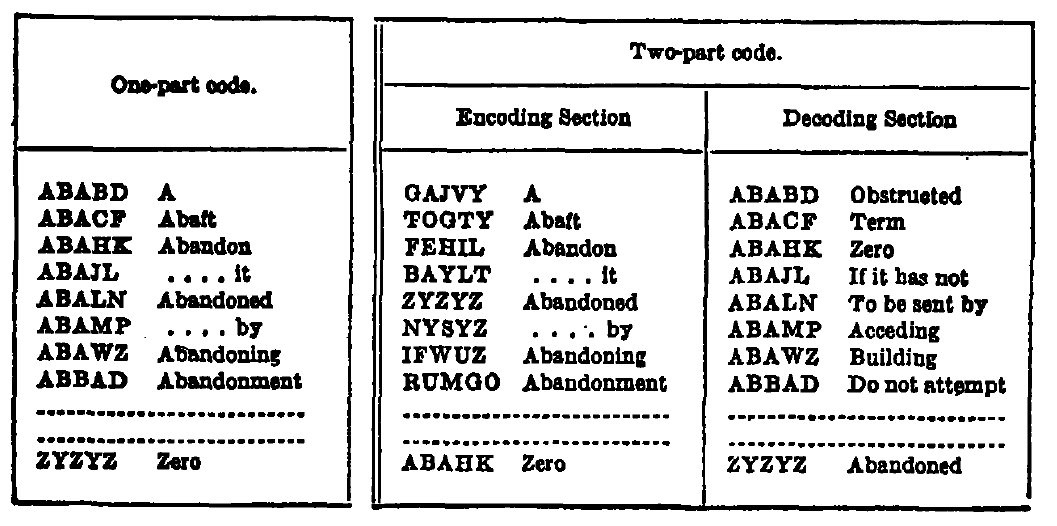
\includegraphics[width=0.9\textwidth,natwidth=1057,natheight=526]{Chapter4_UnnamedFigure.eps}
                \end{figure}
 

\end{enumerate}
\mypara Between the two extremes are codes which have features of both;
that is, complete sections may be arranged in random sequence, but
within each section the contents are arranged in some systematic or
logical order. This is true, however, only of some of the older codes. In
modern types, the two-part construction is more common.


\mypara When a strict alphabetical arrangement is used in the sequence of
the phrases, the code is said to be a strictly alphabetical code; when the
phrases are listed under separate headings based upon the principal word
or idea in the whole expression, the code is said to be a caption code. The
following extracts will serve to illustrate the two types:

\begin{figure}[h]
   \centering
    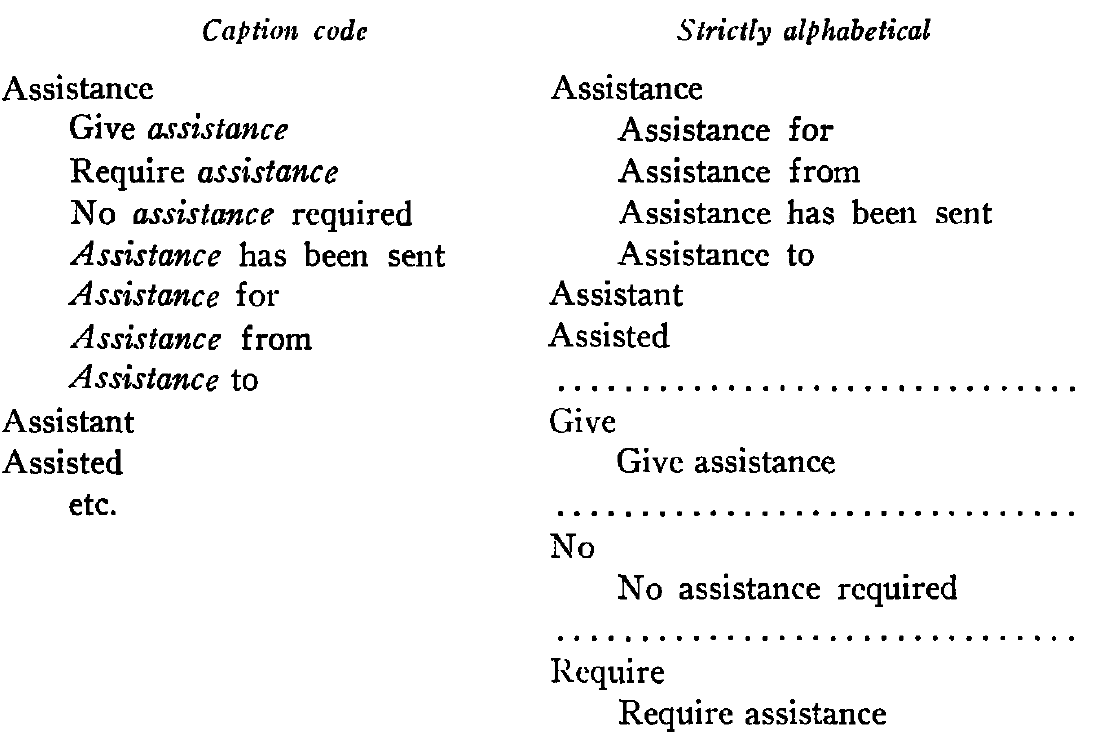
\includegraphics[width=0.9\textwidth,natwidth=1093,natheight=747]{Chapter4_UnnamedFigure2.eps}
\end{figure}

\mypara More precise and economical encoding is possible with a caption
code than with an alphabetical code. With the caption code it is easier
to assemble an extended variety of expressions and shades of meaning
under specific headings than with the alphabetical code. On the other
hand, the use of a caption code involves more time and labor in encoding,
especially by untrained or unskilled personnel, than the use of an alpha-
betical code. Where the phraseology of communication is standardized or
stereotypic, the most common expressions may be listed in an alphabetical
code as readily as in a caption code. In both types of codes there may be
tabulated material, such as tables of numbers, dates, equipment, geographical or personal designations, either fomiing isolated sections in
the code or inserted in the vocabulary under appropriate headings.

\mypara Two-part codes are used by many governments for their secret
diplomatic, military, and naval communications because the advantages
they offer over one-part codes are greater than their disadvantages. The
disadvantages are: a two-part code is harder to handle than a one—part
code because it is at least twice as large in content, since each code group
and each plain—text element must appear twice; the cost of printing is
approximately double; the amount of labor in compiling a two-part code
is nearly four times greater because of the necessity for preparing the
accurate cross—reference arrangement which is its basic principle.

\subsection{Purposes of Two-Part Type of Code}

\mypara The two-part code is a comparatively recent development in code
systems. Its purposes are greater secrecy, and greater accuracy.

\mypara In a one-part code the plain-text groups progress from A to Z in a
regular alphabetical sequence, accompanied by their code groups, also in
a regular alphabetical or numerical sequence. If the word ABAFT is
represented by a code group whose initial letter is A, or whose initial
number is 1, then the word ABANDON will be represented by a group
whose initial letter is also A, or whose initial number is also 1. In other
words, the enemy cryptanalysts have definite clues to follow in breaking
down the code because of the parallelism of the two sequences; the
determination of the value of one code group affords definite clues to the
value of many other code groups. In a two—part code, however, the word
ABAFT might be represented by a group whose initial letter is T, or
whose initial number is 8, and the word ABANDON might be repre-
sented by a code group whose initial letter is F, or whose initial number
is 3. In other words, the two sequences are not alike in progression;
hence the determination of the value of one code group will give no clues
to the value of any other group.

\mypara In considering the greater accuracy of. a two-part code over a one-
part code, the following pair of phrases (in a hypothetical one-part code)
are given as an example:

\begin{verbatim}
WOVAM Will be ready to attack
WOVEN Will not be ready to attack
\end{verbatim}

Such an arrangement is subject to two sources of error. A code clerk
working under great difficulties, in a hurry, may accidentally write down
WOVAM instead of WOVEN as a result of the contiguity of the two
sets of letters which are similar in appearance and are so close together
on the page that his eye may take the group from the wrong line. Again,
on account of the similarity in sound, his ear may deceive him into
writing WOVEN when he should have written WOVAM. Now the
meaning of the one group is the exact opposite of the meaning of the
other and, since either meaning may fit in correctly with the context of
the message, the error may remain undiscovered for some time, thus
causing serious inconvenience or, in the case of combat, actual loss of life.
Furthermore, although the making of two errors in a single group is
rather unusual in transmission or reception, yet it does happen and, in
such a case as the above, would not be detected. This is especially true
in connection with tabular material such as lists of numbers, dates, and
names, in which the context often fails to yield clues to the correction of
garbles or errors, or to give conclusive evidence of the presence of an
error. But in a two-part code such errors are improbable. In the first
source of error mentioned above, the code clerk would be very much less
likely to confuse two entirely different groups of letters; in the second
source, if two errors are made in the transmission or reception, and if
these errors involve two letters producing a group which actually has a
meaning in the code, this meaning is so unlikely to fit in correctly with
the context that its probability of occurrence may be negligible. Thus, if
this sort of error does happen, the meaning of the group fails to fit in
with the context and at once indicates an error. Knowledge of such an
error, even if it is impossible to correct it, is more preferable than
ignorance of its existence, with a possible action based upon incorrect
decodement.

\section{ENCIPHERED CODE}

\subsection{Purposes of Enciphered Code}

\mypara Sometimes the code groups of a code message undergo a further
process of encipherment. The resulting cryptogram constitutes an
enciphered code message.

\mypara It is desirable to use enciphered code in two instances:

\begin{enumerate}
\item When the basic code has had wide distribution and the message
might fall into unauthorized hands. Commercial codes sold in
bookstores, and even special codes distributed widely throughout
governmental offices, illustrate the type of code to which this
added safety factor should be applied.

\item When increased security is necessary for highly classified
communications. Although the basic code book may already be
secret, further encipherment would greatly delay the solution of
the code if it fell into the hands of enemy cryptanalysts.
\end{enumerate}

\mypara It has already been stated that code messages may be solved by
cryptanalytic principles without possession of the code. The length of
time required for the process varies widely, and is dependent upon the
conditions under which the work is done (see ch. 1). To increase the
length of time required for solution, as in secret codes, the code text of
the messages resulting from the use of the code is passed through a
cipher process so that the messages will be in different keys, thus delaying
the assembling and study of data, which is necessary to the solution.

\subsection{Types of Encipherment}

\mypara Both of the two general classes of cipher methods, transposition
and substitution, may be used in enciphering code. The increased degree
of secrecy because of encipherment depends entirely upon the nature of
the system applied.

\mypara Transposition systems involving a rearrangement of complete
groups may be employed where the degree of increased security does act
have to be of a high order, and where the original form of the groups
must be retained even after encipherment. Transposition systems in
which the order of the letters within groups is changed may also be
employed. For example, a numerical key may indicate the transposed
order of the letters of the code groups, so that a group such as XDFGY
will become DFYXG.

\mypara Substitution systems of many sorts may be employed, ranging from
simple monoalphabetic to the most complex types of substitution with
cipher machinery. Tables of alphabets are often used. In some systems,
a simple transposition process may be combined with a simple substitu—
tion process.

\mypara A favorite method in one—part codes having both letter-code and
figure-code groups is that in which the letter-code group standing at a
prearranged interval before or after the letter—code group representing
the actual word or phrase intended to be conveyed is substituted. The
interval may remain fixed within a single message, or it may vary according to some predetermined key. Numerical code groups make the use of
large intervals practicable.

\mypara In modern practice, the most common methods of enciphering
figure-code groups are those using addition or subtraction, with a key
book containing arbitrary groups of figures. When such methods are
properly used, they yield a high degree of security. The highest degree
of security is attained when such a key book is used \textit{only once}.
